\documentclass{article}

\usepackage{amsmath} % math stuff
\usepackage{amssymb} % math stuff
\usepackage{array} % equations and stuff
\usepackage{bm} % bold math
%\usepackage{booktabs} % extra table rule options
%\usepackage{caption} % suppressed table numbering; incompatible with revtex, and longtable, I think
\usepackage{comment} % comment environment
%\usepackage{enumitem} % customization of enumeration, itemize, and description
\usepackage[T1]{fontenc} % font encoding for special characters, must also use scalable font package
\usepackage[margin=0.8in]{geometry} % paper sizes and margins (but be careful not to mess up pre-defined pages)
\usepackage{graphicx} % for graphics
%\usepackage{helvet} % default font is the helvetica postscript font
\usepackage[utf8]{inputenc} % special characters in tex input
\usepackage{layouts} % print units like widths
\usepackage{lipsum} % lorem ipsum filler text
\usepackage{lmodern} % scalable font?
\usepackage{longtable} % multi-page tables
\usepackage{makecell} % specify line-breaks in table cells
\usepackage{mathrsfs} % math script font
\usepackage{mhchem} % easier chemical formula
\usepackage{microtype} % allows disabling of ligatures
\usepackage{multicol} % multicolumns
%\usepackage{newcent} % new century schoolbook font
\usepackage{nicefrac}
\usepackage{numprint} % print and format (large) numbers
\usepackage{parskip} % removes paragraph indentation, and adjusts paragraph skip, as well as list items
\usepackage{pdfpages} % add pdf files as pages
%\usepackage{setspace} % adjust text spacing and indents
\usepackage{siunitx} % decimal alignment
\usepackage{subfigure} % divided figures
%\usepackage{tabu} % extra table options
\usepackage{textcomp} % symbols
\usepackage{threeparttablex} % better footnotes with longtable
\usepackage{titling} % title placement
\usepackage{ulem} % strikethrough text
%\usepackage{url} % superceded by hyperref
\usepackage{verbatim} % verbatim environment
\usepackage{xcolor} % colors and color boxes
\usepackage{xspace} % commands that don't eat up white space
\usepackage{hyperref} % links and page setup; should always come last

\hypersetup{
 bookmarks=true,
 colorlinks=true,
 citecolor=blue,
 linkcolor=blue,
 urlcolor=blue,
 pdfstartview={XYZ null null 1.0} % default open view is 100%
}

\DisableLigatures[f,t]{encoding = T1} % disable ff, fi, fl, tt ligatures; without options, it also disables -- = endash
\renewcommand{\arraystretch}{1.0} % extra vertical (and horizontal?) space in tables

% define centered, left- and right-aligned columns with specified widths
\newcommand{\PreserveBackslash}[1]{\let\temp=\\#1\let\\=\temp}
\newcolumntype{C}[1]{>{\PreserveBackslash\centering}p{#1}}
\newcolumntype{L}[1]{>{\PreserveBackslash\raggedright}p{#1}}
\newcolumntype{R}[1]{>{\PreserveBackslash\raggedleft}p{#1}}

\begin{document}

\pagestyle{empty} % don't number pages

% custom title
\begin{center}
{\LARGE Express Riddler}

\vspace{0.15in}

{\Large 23 July 2021}
\end{center}


\section*{Riddle:}

The following 8-by-8 grid is covered with a total of 64 chess pieces, with one piece on each square.
You should begin this puzzle at the white bishop on the green square.
You can then move from white piece to white piece via the following rules:

\begin{itemize}
\item If you are on a pawn, move up one space diagonally (left or right).
\item If you are on a knight, move in an ``L'' shape---two spaces up, down, left or right, and then one space in a perpendicular direction.
\item If you are on a bishop, move one space in any diagonal direction.
\item If you are on a rook, move one space up, down, left or right.
\item If you are on a queen, move one space in any direction (horizontal, vertical or diagonal).
\end{itemize}

\begin{center}
\vspace{0.1in}
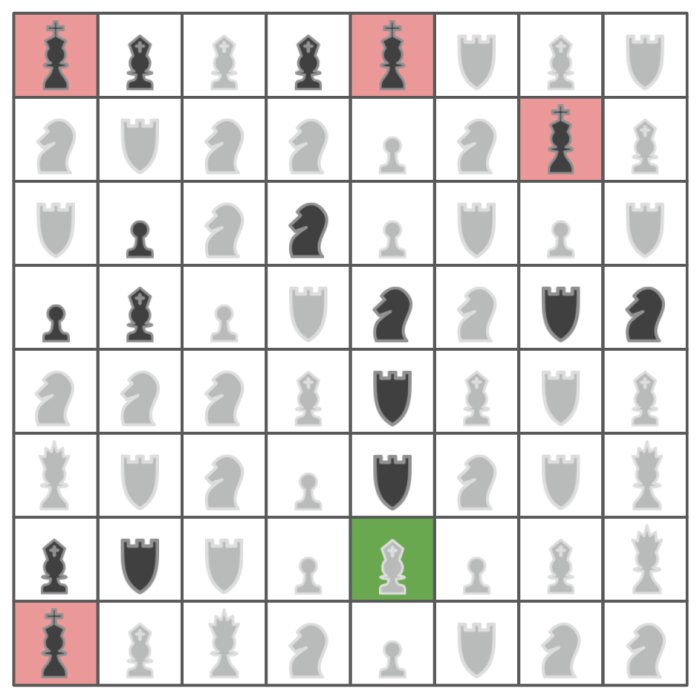
\includegraphics[width=3in]{chess.png}
\vspace{0.1in}
\end{center}

For example, suppose your first move from the bishop is diagonally down and to the right.
Now you're at a white rook, so your possible moves are left or up to a pawn or right to a knight.

Your objective is to reach one of the four black kings on the grid.
However, at no point can you land on any of the other black pieces.
(Knights are allowed to hop over the black pieces.)

What sequence of moves will allow you to reach a king?



\section*{Solution:}

Here is my solution.
I'm sure it's not the only solution, and I have no idea if it's the shortest solution.

\begin{center}
\vspace{0.1in}
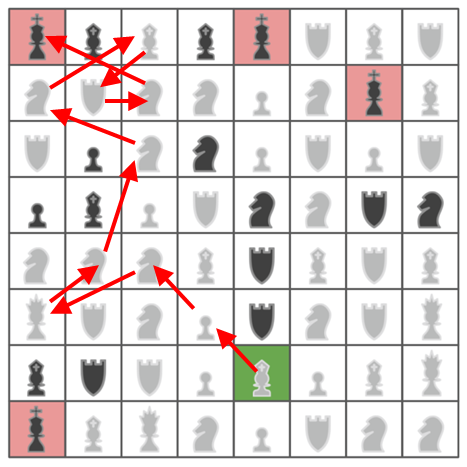
\includegraphics[width=3.5in]{chess_complete.png}
\end{center}




\end{document}